\documentclass{standalone}

\usepackage{xcolor}
\usepackage{bm}
\newcommand{\mat}[1]{\bm{#1}}

\usepackage{tikz}
\usepackage{tikz-3dplot}

\begin{document}

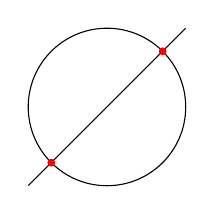
\begin{tikzpicture}
\draw (0,0) circle [radius=1];
\draw (-1,-1) -- (1,1);
\fill[red] (-0.7071,-0.7071) circle [radius=0.5mm];
\fill[red] (0.7071,0.7071) circle [radius=0.5mm];

\end{tikzpicture}
\end{document}
